\documentclass[11pt]{article}

\usepackage{common}
\usepackage{booktabs}
\title{Practical 1: Regression \\ Predicting the Efficiency of Organic Photovoltaics}
\author{Antonio (email, Camelot.ai username) \\
	Fangli (fgeng@g.harvard.edu, Camelot.ai fangligeng) \\
	Xihan (xihanzhang@hsph.harvard.edu, Camelot.ai Xihan)}
\begin{document}


\maketitle{}


%\noindent This is the template you should use for submitting your practical assignments. A full-credit assignment will go through each of these points and provide a thoughtful clear answer.  Note that the limit for the report is 4 pages, please prioritize quality over quantity in your submission.

\section{Technical Approach}

We began by performing exploratory analysis on the sample dataset we were given, which consisted of a training set of 1 million molecules with 256 binary predictors, in addition to their SMILES string and the HOMO--LUMO gap we were seeking to predict. The test set consisted of 824,230 molecules with the same set of predictors as well as their SMILES string. The sample code we were given implemented a default Linear Regression model on the full set of 256 predictors, yielding an $R_\textrm{LR}^2 = 0.461 (\textrm{MSE}_\textrm{LR} = 0.089)$ over the full training set, and a default Random Forest regression with $R_\textrm{RF}^2 = 0.554 (\textrm{MSE}_\textrm{RF} = 0.074)$.

Initial inspection found that out of 256 molecular features, 221 of them were unexpressed (i.e. had $x_i = 0$) for \emph{all} molecules, both in the training set and the test set. Dropping unimportant features would normally call for $K$-fold cross-validation across the training set to ensure those features are consistently unimportant in all cases. However, in the case of null values of certain features for every element of the training set, it is not only legitimate but necessary to drop those features from all further analysis, as fitting along null dimensions would constitute a form of overfitting.

Having reduced the sample dataset to 31 expressed molecular features, we performed both regularized and non-regularized linear regression with cross-validation\footnote{After initially trying 3-fold, 5-fold and 10-fold cross-validation, we settled on 5-fold cross-validation as the best compromise between accuracy and computational speed.} and hyperparameter tuning, under the following methods:

\begin{enumerate}

\item Non-regularized linear regression: Yields $R^2 =  ...$
\item Ridge Regression: 
\item Lasso:
\item Elastic Net:

\end{enumerate}

The results from linear regression on the sample dataset consistently gave us low predictive value, even when compared to generic random forest regression, which led us into pursuing 2 parallel tracks:

\begin{enumerate}

\item Non-linear methods: 

Among these we concentrated on 2 broad categories:

\begin{enumerate}

\item Tree-based Ensemble methods: 
Given all the predictors are binary, which is coincide with the branch-like structure of decision tree--nodes as the predictors and samples as leaves, we had a deeper dive into decision tree. Single tree always choose the cutpoint to split the predictor space into two regions that leads to the greatest possible reduction in RSS(given by $\sum_{J}^{j=1}\sum_{i\in R_{j}}(y_{i}-\hat{y_{R_{j}}})^{2}$, where $\hat{y_{R_{j}}}$ is the mean prediction within the leaf)\footnote{An Introduction to Statistical Learning} . Thus, the more branch a tree has, the more precise the predcition would be. However, this deep-depth tree may overfit the training set and have high varriance among all trees. This is why we choose to fit ensemble methods, that can combine many trees and take the average of prediction made by each individual tree. 
The baseline ensemble methods we tried for the first step are:
\begin{enumerate}
\item Bagging (\emph{sklearn.ensemble.BaggingRegressor}): The strategy for bagging to reduce the variance is to boostrap multiple training sets to fit multiple trees.
\item Randomforest (\emph{sklearn.ensemble.RandomForestRegressor}): Random Forest further reduce the variance by randomly pick sub set of $\mathit{m}$ (usually $\sqrt{p}$) predictors from the total predictors(the number is $\mathit{p}$) at each split to make, so that all the trees would have less similar structure compared with bagging trees.
\item Extremely Randomized Trees (\emph{sklearn.ensemble.ExtraTreesRegressor}): Extremely Randomized Trees even futher reduce the variance by select predictor from the $\mathit{m}$ predictors totaly at random(rather than prefer those have higher split effciency). 
\item AdaBoost (\emph{sklearn.ensemble.AdaBoostRegressor}): Adaboost takes a different strategy, which is to use a linear combination of multiple simple trees to reduce the residual step by step (essentially focus more on bias). 
\end{enumerate}
To reduce the computaion load, we fit the baseline models on the 31 features after filtering. We splitted 20\% of the training set as validation set to test MSE generated by each model and found the performance of Bagging, Randomforest, Extremely Randomized Trees are quit similar to each other, while Adaboost is much weaker. 

This is essentially because Adaboost focus more on reducing bias and the other 3 methods focus on reducing varriance. From this we can draw conclusion that, we can focus more on tuning those hyper parameters that can efficiently reduce variance of the model. The MSE of the 4 models are as below: 

\begin{figure}[h]
\centering
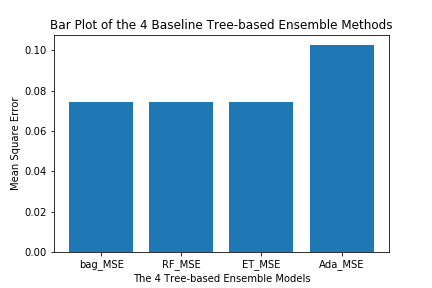
\includegraphics[width=0.6\textwidth]{MSE_ensemble}
\caption{Bar Plot of the 4 Baseline Tree-based Ensemble Methods}
\label{fig:MSE_ensemble}
\end{figure}



Then we select random forest as main model to tune, and we use 5-fold cross validation to tune number of estimators (i.e. the total number of trees to take average on, which is key to reduce variance) on the newly generated predictor space with 2048 features within 1/7 of the total sample. 

Here we met up with a variance-computaional complexity trade-off, that is: the more estimators we use, the less varriance of random forest suffers from. Given the computational resources we have(fitting 1 random forest on full data set takes more than 5 hours), and given the total sample size is 7 times of the test set we tune the model(where number of estimator=10 has reasonable performance), setting the number of estimators to be 150 for the whole data set is safe and reasonable. 
Since the sample size is much larger than feature size, even though the max depth equal to total number of features, each leaf still contain more than 500 samples, we didn't put computational resources on tuning max depth of each tree.

We also plot the distribution of importance of predictors based on the baseline random forest, the result is as below:

\begin{figure}[h]
\centering
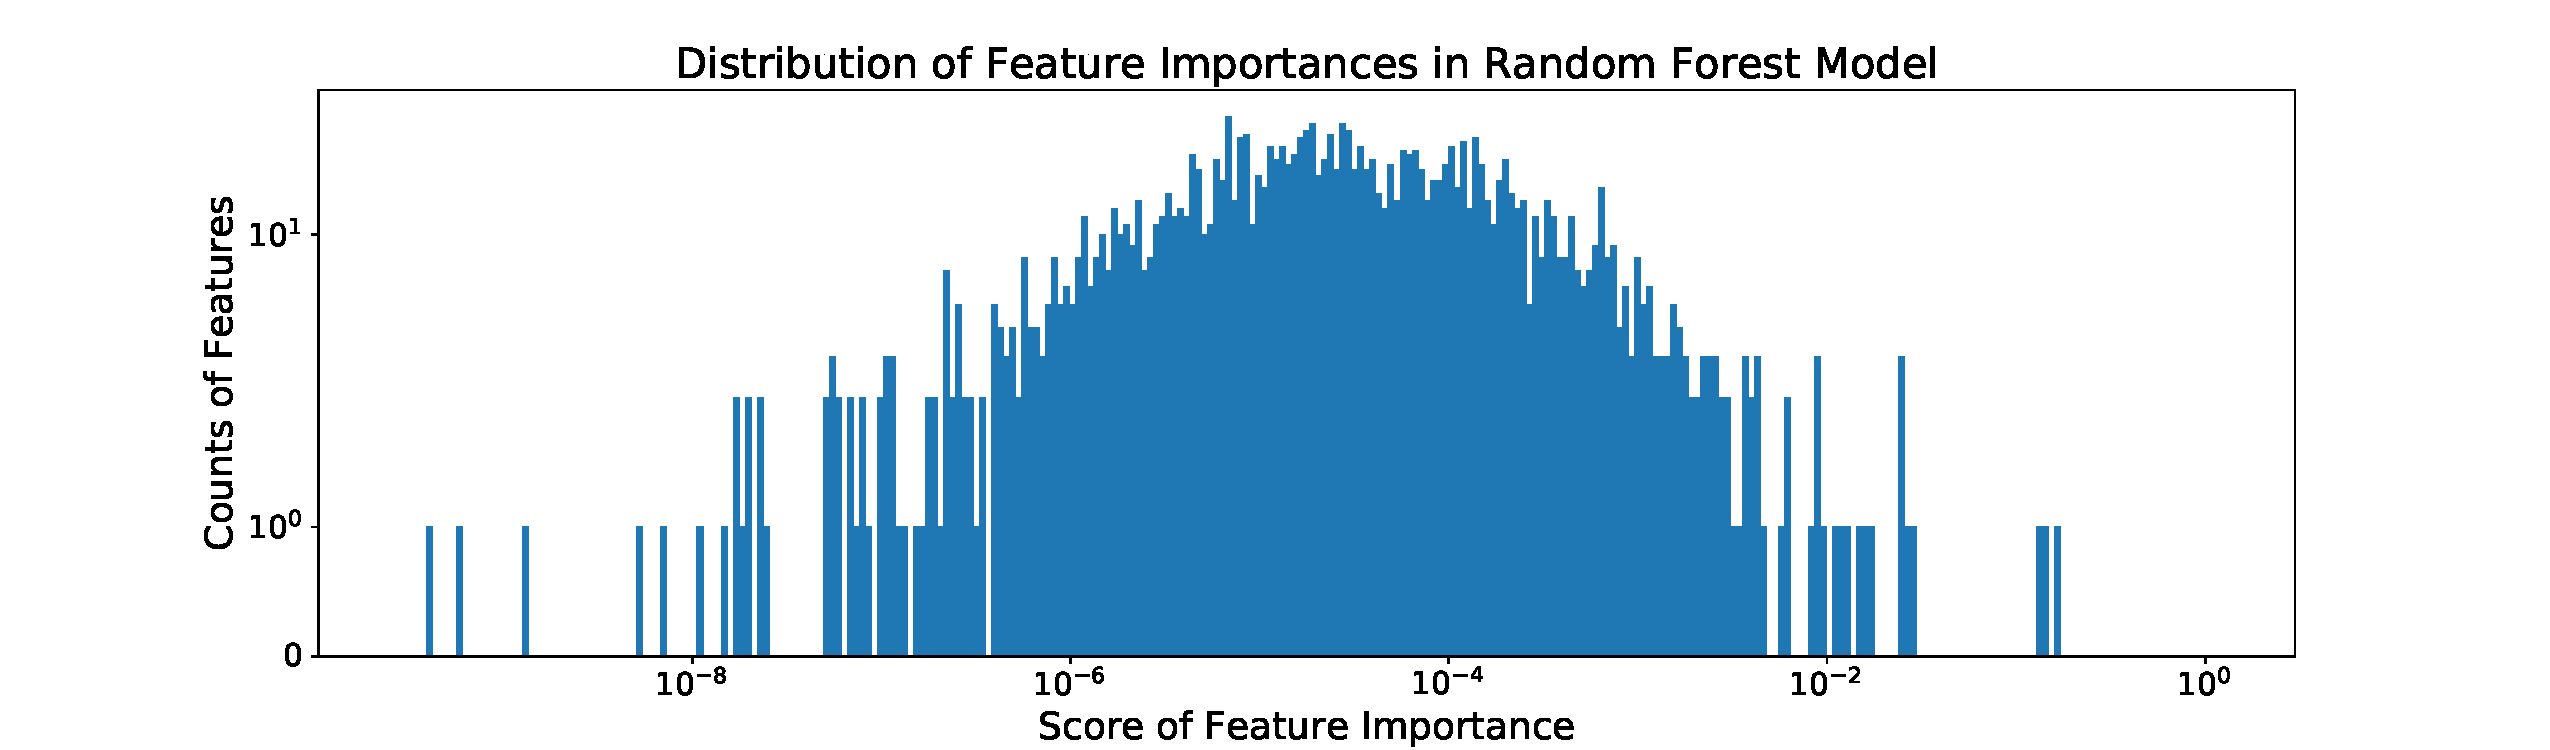
\includegraphics[width=\textwidth]{his_feature_importance}
\caption{Histogram of feature importances from Random Forest}
\label{fig:his_feature_importance}
\end{figure}

We can see most portion of predictors have little importance($10^-8$ to $10^-2$), but combining them together would yield good precision on validtion set($R^2 = 0.936$, MSE=0.0106). This made us explore more on Deep learning method, which considers the interaction among features.

\item Deep learning: Since the predictors describe a broad set of molecular properties, it is natural to expect non-linear interactions between them to play a role in determining the HOMO--LUMO gap. For this reason we decided to explore the training of simple neural networks that would serve to model these interactions and got acquainted with the basics of Deep Learning as a tool to tackle this problem. In all cases, we used an architecture of one or more dense (fully-connected) hidden layers between the input layer of $N$ parameters and the output layer of 1 node for the response we wanted to model. For each node in the hidden layers, we used the widely used ``relu'' function ($f(x \le 0) = 0, f(x > 0) = x$) as activation function. We trained the model using the \emph{keras} module in Python, using the \emph{adam} optimizer for the learning rate, and setting aside 20\% of training data for validation. The model would be fitting for the weights of the connections between pairs of nodes in the network, which in the case of 1 hidden layer with $M$ nodes, would result in $(N + 1) \times M$ parameters to be trained.

Taking a trial-and-error approach to setting the network architecture, we show the results of validation set MSE for 3 broad cases, using the 31 expressed features in the sample training dataset: 1) 1 hidden layer with variable number of nodes, 2) 2 hidden layers, with 31 nodes on the first and variable number of nodes on the second, and 3) 3 hidden layers, with 31 nodes on each of the first two, and variable number of nodes on the third.

\emph{Figure with 3 plots for 1, 2 and 3 hidden layers}

The result of this experiment showed that the MSE was not as sensitive to the addition of a second and third layer, as it was to the number of nodes in the first layer of the 1-hidden layer architecture. Given the computational limitations that were expected for a much larger set of features, we used this result to use the feature-engineered set to train only 1-layer models with a limited number of nodes in the same range as the number of predictors.


\end{enumerate}
\item Feature engineering: 

Based on the regression, random forest and deep learning neural models we trained on original dataset, we found that those 256 features didn't yield as good results as we expected. Therefore, we were thinking how much improvement we could get by adding more information and went to explore the molecule strings and RDKit package in Python. \\

RDKit provides all different kinds of information and functions about a molecule by recognizing its SIMLES strings, including substructure searching, chemical reaction, enumeration of molecular resonance structures, and several sorts of fingerprints. After our research, we decided to extract Morgan fingerprint function,as it is widely used with SKLearn in Machine Learning and it carries the information which we think is most relevant to the efficiency of organic photovoltaics. \\ 

The information that Morgan fingerprint provides is displayed below:
\begin{enumerate}
\item Connectivity: Element, numbers of heavy neighbors, numbers of Hs, charge, isotope, inRing
\item Chemical features: Donor, Acceptor, Aromatic, Halogen, Basic, Acidic
\item Taking into account the neighborhood of each atom\\
\end{enumerate}
The process is first taking the "SMILES" column from the training and test data and using RDKit to convert it into molecule objects. Then for each molecule object, we implemented command {\itshape rdkit.Chem.getmorganfingerprintasbitvect()} to get Morgan fingerprint. After iterate this process for each string, we appended the columns together to form a new input matrix. During Morgan fingerprint extraction process, We mainly adjusted the parameter "nBits" to 512, 2048 and 4096 aiming to test datasets with various preciseness levels. As preciseness level increases, the size of dataset also increase largely. Due to the computational constraints, we decided to slice the datasets into 7 parts in order to reuse and avoid the memory crash. \\

\end{enumerate}

\section{Results}
Table 1 displays the performance of models we tested after we got the new feature information from RDKit. 

\begin{table}[h]
\centering
\begin{tabular}{llr}
 \toprule
 Model &  & RMSE \\
 \midrule
 \textsc{linear regression w/ 2048 features} & & 0.12364\\
 \textsc{linear regression w/ 429 features} & & 0.16869 \\
 \textsc{random forest w/ 2048 features} & & 0.06435 \\
 \textsc{neural network w/ 2048 features w/ 2 layers and 100 units in each layer} & & 0.03564  \\
 \textsc{neural network w/ 2048 features w/ 1000 units} & &0.03553 \\
 \textsc{neural network w/ 4096 features w/ 1024 units} & & 0.03461\\
 \bottomrule
\end{tabular}
\caption{\label{tab:results} MSE of models tested using new feature information from RDKit}
\end{table}

\begin{enumerate}
\item Feature set selection

To select best feature set, we test the performance of the model we have experimented on as mentioned in Technical Approach: 
\begin{enumerate}
\item Linear Regression

We first used 2048 features (which is default in RDKit function) and tested the linear regression. Its results gave us a better result (RMSE 0.1236) than that the best deep learning model (Antonio please put a number here) gave us with 256 features. It indicates the big loss of information using 256 features. \\
For the purpose of further exploration and reduction of computational burden, we tried to drop the features which have coefficient = 0 from linear regression model results, however, only 1\% of the 2048 features can be dropped. We increased the threshold of dropping data until abs(coefficient)<=0.15, this finally gave a subset with 429 features. We then ran linear regression again with the new subset, but the final RMSE was increased by 30\%. 

\item Random Forest

We also ran random forest model with 512 features and 2048 features, but it showed that the 2048 features result was much better than the others. 
\end{enumerate}

These two sets of comparison demonstrated that either 429 features selected by linear regression coefficient or 512 features directly given by RDKit fingerprint function was not informative enough. Therefore, we decided to test tune different models with 2048 features, which give us a relatively good amount of information for the molecules energy efficiency prediction. \\

\item Tuning on neural network

As discussed in the technical approach part, the experiments using original dataset (256b features) show that neural network with one layer could provide the most accurate results. So we decided to test neural network model With 2048 features. 

We set up 3 different configurations to conduct the experiments with neural network: 
\begin{enumerate}
\item 2 layer neural network with 2048 features and 100 units in each layer; 
\item 1 layer neural network with 2048 features with 1000 units; 
\item 1 layer neural network with 4096 features with 1024 units. 
\end{enumerate}
Comparing the results between 1st and 2nd experiment, we found the layer number is not as important as unit number, which is consistent with what we found using the smaller number of features. Comparing the result between 2nd and 3rd experiment, we found that 2048 Morgan fingerprint is basically informative enough to predict, and 4096 features in more detail couldn't improve the prediction as much but meanwhile taking a much larger amount of time for computation.

As 4096 features with 1 layers and 1024 nodes didn't provide the prediction as precise as we expected, we were turning to find additional features and found counted-based fingerprints could be a good option in addition to the bit-based fingerprint we used. Count-based fingerprint count the number of times a feature appears instead of simply that it appears, which could potentially provided new and important information to our prediction. \\

\item Other methods not realized

We also wanted to try other algorithms like Principal Component Analysis to select more important features to reduce computational complexity, and to implement neural network models with 2 layer and 2000 nodes to allow more complex interactions between selected important features. However, due to the time constraints we had, we didn't realize those plans. \\

\item Summary

As a summary, we found that the linear regression and random forest are good methods to rapidly select useful features. Neural network is much more accurate in non-linear regression, especially with large dataset and rich features condition. \\


\item Box Plots for the performance of other tested models

(Antonio): Main result here should be a box plot with the MSE of different methods we tried. Models for the original data (256 features) should be different from models for the dataset of all the features.
\end{enumerate}

\section{Discussion} 

{\itshape
End your report by discussing the thought process behind your
analysis. This section does not need to be as technical as the others 
but should summarize why you took the approach that your did. Credit will be given for:

  \begin{itemize}
  \item Explaining the your reasoning for why you seqentially chose to
    try the approaches you did (i.e. what was it about your initial
    approach that made you try the next change?).  
  \item Explaining the results.  Did the adaptations you tried improve
    the results?  Why or why not?  Did you do additional tests to
    determine if your reasoning was correct?  
  \end{itemize}
 }

\end{document}

